%% ----------------------------------------------------------------
%% Thesis.tex -- MAIN FILE (the one that you compile with LaTeX)
%% ---------------------------------------------------------------- 

% Set up the document
\documentclass[a4paper, 11pt, oneside]{uet_thesis}  % Use the "Thesis" style, based on the ECS Thesis style by Steve Gunn
\graphicspath{{Figures/}}  % Location of the graphics files (set up for graphics to be in PDF format)

% Include any extra LaTeX packages required
\usepackage[square, numbers, comma, sort&compress]{natbib}  % Use the "Natbib" style for the references in the Bibliography

\usepackage{verbatim}  % Needed for the "comment" environment to make LaTeX comments
\usepackage{vector}  % Allows "\bvec{}" and "\buvec{}" for "blackboard" style bold vectors in maths
\usepackage{url}
\usepackage{natbib}
\usepackage{enumitem}
\usepackage{float}

\hypersetup{urlcolor=blue, colorlinks=true}  % Colours hyperlinks in blue, but this can be distracting if there are many links.

% remove the unnecessary spacing before and after the headings/subheadings
\usepackage[compact]{titlesec}
\titlespacing{\section}{0pt}{*0}{*0}
\titlespacing{\subsection}{0pt}{*0}{*0}
\titlespacing{\subsubsection}{0pt}{*0}{*0}

\setlength{\parskip}{6pt}
%\setlength{\parsep}{0pt}
%\setlength{\headsep}{0pt}
%\setlength{\topskip}{0pt}

%% ----------------------------------------------------------------
\begin{document}
\frontmatter	  % Begin Roman style (i, ii, iii, iv...) page numbering

% Set up the Title Page
\title  {Efficient H.264 Encoder with Main Profile for High Frame Rate Video Streams}
%\session {2019 -- 2023}
\advisor {Dr. Muhammad Tahir}
\authors {
Fariaa Faheem ~~~~~ 2019-EE-001\\
Marwa Waseem ~~~~~ 2019-EE-007\\
Hamza Akhtar ~~~~~ 2019-EE-012\\
Filza Shahid ~~~~~ 2019-EE-151
}

\addresses  {\deptname \\ \univname}  % Do not change this here, instead these must be set in the "Thesis.cls" file, please look through it instead
\date       {\today}
\subject    {}
\keywords   {}

\maketitle
%% ----------------------------------------------------------------

\setstretch{1.3}  % It is better to have smaller font and larger line spacing than the other way round

% Define the page headers using the FancyHdr package and set up for one-sided printing
\fancyhead{}  % Clears all page headers and footers
\rhead{\thepage}  % Sets the right side header to show the page number
\lhead{}  % Clears the left side page header

\pagestyle{fancy}  % Finally, use the "fancy" page style to implement the FancyHdr headers


%% Select only one of the certification pages  
%\CertificationMSc{}
\CertificationBSc{}
\clearpage  % Certification ended, now start a new page


%% ----------------------------------------------------------------
% Declaration Page required for the Thesis, your institution may give you a different text to place here
\Declaration{
%\addtocontents{toc}{\vspace{1em}}  % Add a gap in the Contents, for aesthetics

I declare that the work contained in this thesis is my own, except where explicitly stated otherwise. In addition this work has not been submitted to obtain another degree or professional qualification.

\bigskip

Signed:~~ \rule[0em]{10em}{1.0pt} \\ % This prints a line for the signature 
Date:~~~~ \rule[0em]{10em}{1.0pt}  % This prints a line to write the date
}
\clearpage     % Declaration ended, now start a new page

%% ----------------------------------------------------------------

\setstretch{1.3}  % Reset the line-spacing to 1.3 for body text (if it has changed)

% The Acknowledgements page, for thanking everyone
\acknowledgements{
%\addtocontents{toc}{\vspace{1em}}  % Add a gap in the Contents, for aesthetics

We would like to express our sincere gratitude to our supervisor Dr. Muhammad Tahir and co-supervisor Sir Umer Shahid, for their unwavering support and guidance throughout this project. We would like to thank Ms. Shehzeen Malik for her advice, constructive criticism and assistance in keeping
our progress on schedule. We would like to acknowledge the contribution of our friends and families for their support during the development of project.

}
\clearpage  % End of the Acknowledgements

%% ----------------------------------------------------------------

% Begin the Dedication page
\setstretch{1.3}  % Return the line spacing back to 1.3
\pagestyle{empty}  % Page style needs to be empty for this page
\dedicatory{Dedicated to our families.}

\clearpage 	% End of the Dedication
%% ----------------------------------------------------------------

% Begin the Sustainable Development Goals page
\setstretch{1.3}  % Return the line spacing back to 1.3
\pagestyle{plain}  % Page style needs to be empty for this page

\addtotoc{Contribution to Sustainable Development Goals}
\vspace{0.5in}
\begin{center}
	\huge{\bf Contribution to Sustainable Development Goals} 
	\par
\end{center}

\vspace{0.5in}
Our project is a part of a long term project of \textbf{Open Eyes}. The idea is to develop a main RISC-V based processor, a video processor, ISP and integrate them on ChipYard to fabricate an IC. This project goes beyond sustainability by tackling the issue of data storage and security in the camera industry. Security camera manufacturers often retain the data collected by their cameras on the servers and then analyze it. This practice is alarming as it raises concerns about the data privacy, potential misuse of data and breach susceptibility.

Every thing related to camera is being developed from scratch under this project, this eliminates the risk of data misuse by any third party data storage and enhances data security. Our strategy will ensure that the data stays in the hands of the camera owners. This will empower the camera industry and the audience of it by putting privacy, security, and data sovereignty as top priorities that contribute to sustainable practices.

Our project will also empower the organizations and individuals to maintain a high level of trust in the camera technology they use and to  make informed decisions about their data. 

\clearpage	% End of the Sustainable Development Goals
%% ----------------------------------------------------------------

\pagestyle{fancy}  %The page style headers have been "empty" all this time, now use the "fancy" headers as defined before to bring them back

%% ----------------------------------------------------------------
\lhead{\emph{Contents}}  % Set the left side page header to "Contents"
\tableofcontents  % Write out the Table of Contents

%% ----------------------------------------------------------------
\lhead{\emph{List of Figures}}  % Set the left side page header to "List if Figures"
\listoffigures  % Write out the List of Figures

%% ----------------------------------------------------------------
\lhead{\emph{List of Tables}}  % Set the left side page header to "List of Tables"
\listoftables  % Write out the List of Tables

%% ----------------------------------------------------------------
\setstretch{1.5}  % Set the line spacing to 1.5, this makes the following tables easier to read
\clearpage  % Start a new page
\lhead{\emph{Abbreviations}}  % Set the left side page header to "Abbreviations"
\listofsymbols{ll}  % Include a list of Abbreviations (a table of two columns)
{
% \textbf{Acronym} & \textbf{W}hat (it) \textbf{S}tands \textbf{F}or \\
\textbf{AVC} & \textbf{A}dvance \textbf{V}ideo \textbf{C}oding \\
\textbf{MB} & \textbf{M}acro \textbf{B}lock  \\
\textbf{VBS} & \textbf{V}ariable \textbf{B}lock \textbf{S}ize \\
\textbf{PE} & \textbf{P}rocessing \textbf{E}lement \\
\textbf{ME} & \textbf{M}otion \textbf{E}stimation  \\
\textbf{FBS} & \textbf{F}ixed \textbf{B}lock \textbf{S}ize \\
\textbf{MV} & \textbf{M}otion \textbf{V}ector \\
\textbf{DCT} & \textbf{D}iscrete \textbf{C}osine \textbf{T}ransform \\
\textbf{QP} & \textbf{Q}uantization \textbf{P}arameter  \\
\textbf{FS} & \textbf{F}ull \textbf{S}earch  \\
\textbf{CAVLC} & \textbf{C}ontext \textbf{A}daptive \textbf{V}ariable \textbf{L}ength \textbf{C}oding \\
\textbf{RAM} & \textbf{R}ead \textbf{O}nly \textbf{M}emory \\
\textbf{NAL} & \textbf{N}etwork \textbf{A}bstraction \textbf{L}ayer \\
\textbf{VCL} & \textbf{V}ideo \textbf{C}oding \textbf{L}ayer \\
%\textbf{SPS} & \textbf{S}equence \textbf{P}arameter \textbf{S}ets \\
%\textbf{PPS} & \textbf{P}icture \textbf{P}arameter \textbf{S}ets \\
\textbf{CBP} & \textbf{C}oded \textbf{B}lock \textbf{P}attern \\
\textbf{FPGA} & \textbf{F}ield \textbf{P}rogrammable \textbf{G}ate \textbf{A}rray \\
%\textbf{FDCT} & \textbf{F}orward \textbf{D}iscrete \textbf{C}osine \textbf{T}ransform \\
\textbf{DFT} & \textbf{D}iscrete \textbf{F}ourier \textbf{T}ransform \\
\textbf{DST} & \textbf{D}iscrete \textbf{S}ine \textbf{T}ransform \\
%\textbf{DWT} & \textbf{D}iscrete \textbf{W}avelet \textbf{T}ransform \\
%\textbf{WHT} & \textbf{W}alsh \textbf{H}adamard \textbf{T}ransform \\
\textbf{QP} & \textbf{Q}uantization \textbf{P}arameter \\
}

%% ----------------------------------------------------------------
% The Abstract Page
\addtotoc{Abstract}  % Add the "Abstract" page entry to the Contents
\abstract{
%\addtocontents{toc}{\vspace{1em}}  % Add a gap in the Contents, for aesthetics
The Thesis Abstract is written here (and usually kept to just this page). The page is kept centered vertically so can expand into the blank space above the title too\ldots

}
\clearpage  % Abstract ended, start a new page

%% ----------------------------------------------------------------
\mainmatter	  % Begin normal, numeric (1,2,3...) page numbering
\pagestyle{fancy}  % Return the page headers back to the "fancy" style
\onehalfspacing
% Include the chapters of the thesis, as separate files
% Just uncomment the lines as you write the chapters

% Chapter 1

\chapter{Introduction} % Write in your own chapter title
\label{Chapter1}
\lhead{Chapter 1. \emph{Introduction}} % Write in your own chapter title to set the page header

Digital video refers to a sequence of images displayed on a screen at a predetermined rate. The process of transferring video content from one medium to another depends on both the duration of the video and the size of the encoded bits. \textbf{Video compression} techniques are commonly utilized to reduce the overall size of the video, which consequently leads to a decrease in the amount of data required for transmission and storage of digital video signals.

The most current video coding standard is known as \textbf{H.264/AVC or MPEG-4 Part-10}. This standard was jointly developed by the \textbf{ITU-T Video Coding Experts Group} and \textbf{ISO/IEC JTC 1 Moving Picture Experts Group}. Compared to typical video coding standards, H.264/AVC provides significantly higher efficiency, capable of reducing bit rate requirements by up to 50$\%$ while maintaining the same level of video quality. It is designed to cover a wide range of video resolutions, from QCIF to HDTV \cite{lin2008parallel}.


% explain the h.464 profiles and levels 
\section{H264 Profiles}
The H.264 family of standards includes various capabilities. These profiles are mainly used to reduce the frame count by implementing motion prediction and temporal compression \cite{rgb-h264-profiles}. The most common ones are:

\begin{itemize}
	\item Baseline Profile
	\item Main Profile
	\item High Profile
\end{itemize}

\subsection{Baseline Profile}
In the realm of video encoding, baseline profiles are commonly employed in applications that require low-power consumption and cost-efficiency. These profiles are capable of achieving an impressive compression ratio of 1000:1, resulting in a streamlet of 1 Gbps being compressed down to approximately 1 Mbps. Baseline profiles utilize a 4:2:0 chrominance sampling method, whereby color information is sampled at half the vertical and horizontal resolution of the black-and-white information. This technique enables the reduction of data without significantly impacting the overall quality of the video.

Furthermore, Universal Variable Length Coding (UVLC) and Context Adaptive Variable Length Coding (CAVLC) are employed as the primary entropy encoding techniques within this profile. Such encoding methods contribute significantly to the efficient compression of video data, while ensuring that the encoded video stream is in compliance with relevant standards. 

\subsection{Main Profile}
Significant enhancements were made to the Baseline Profile through the introduction of advanced frame prediction algorithms, resulting in the development of the Main Profile. This updated profile is primarily utilized for standard-definition digital TV broadcasts in MPEG-4 format.

However, it should be noted that the Main Profile is not employed in high-definition broadcasts. Rather, alternate profiles are used in such scenarios to ensure optimal video quality and compatibility with relevant standards.

\subsection{High Profile}
Introduced in the year 2004, the High Profile is considered to be the most efficient and powerful profile within the H.264 family. It is primarily utilized in high-definition television applications such as Blu-ray Disc storage, Digital Video Broadcasting (DVB) and HDTV broadcast services. This profile is capable of achieving an exceptional compression ratio of 2000:1, which is a significant improvement over previous encoding standards. It utilizes an adaptive transform method that allows for the selection of either 4x4 or 8x8 pixel blocks. This enables preservation of video quality while reducing network bandwidth consumption by up to 50$\%$.

Furthermore, the application of this compression technique facilitates the compression of a 1 Gbps stream to approximately 512 Kbps, further emphasizing the impressive capabilities of the High Profile.

The overall procedure of H.264 includes various components. The top level block diagram of an H.264 Encoder is shown in Figure \ref{fig:toplevel}.

\begin{figure}[htbp]
	\centering
	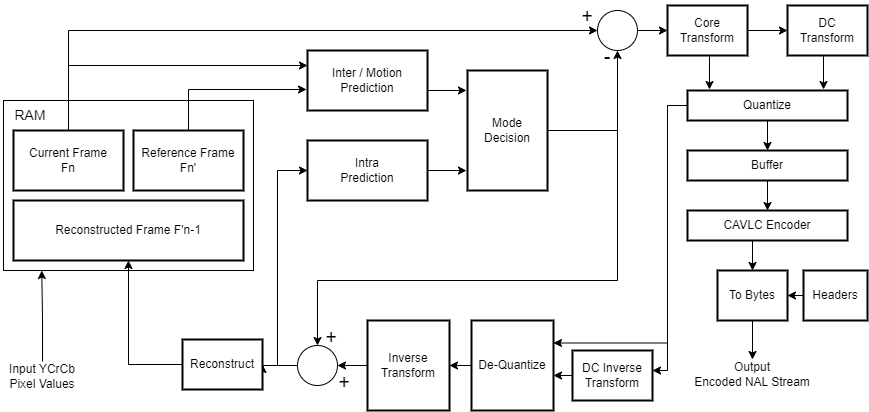
\includegraphics[width = 5in]{./Figures/toplevel.png}
	\rule{35em}{0.5pt}
	\caption{Top Level Diagram for H.264 Encoder}
	\label{fig:toplevel}
\end{figure}

% explain the components briefly
\section{H264 Process}
An H264 encoder has a \textbf{forward path} and a \textbf{reconstruction path} \cite{sahin2006efficient}. The forward path uses \textbf{intra} and \textbf{inter predictions} to encode a video frame to create a bit stream. The reconstruction path is used to decode the encoded frame and to reconstruct the decoded frame. Reconstruction path in encoder ensures that both encoder and decoder make use of similar reference frames for inter and intra prediction. This is to avoid encoder-decoder mismatches. 

\subsection{Forward Path}
The input frame is partitioned into \textbf{Macro-Blocks (MB)}. These MB are then encoded in intra or inter mode. This depends on mode decision. The current MB is predicted from reconstructed frame. This predicted MB is generated by intra prediction based on \textbf{spatial redundancy}, and by inter prediction based on \textbf{temporal redundancy}. The mode is chosen based on better quality and bit rate performance of these 2 modes. The Predicted MB is subtracted from current MB to create a \textbf{Residual MB}. Residual data is \textbf{transformed} (4x4 integer transform), then \textbf{quantized}. The obtained coefficient are re-ordered in a \textbf{zig-zag order} which are regarded as \textbf{entropy encoded}. These coefficients along with header information form the \textbf{compressed bit stream}. This stream is forwarded to NAL for storage or transmission. 

\subsection{Reconstruction Path}
This path takes quantized transform coefficients and performs inverse quantization and inverse transform. In this way, reconstructed residual data is generated, but they are not identical to original residual data as quantization is a lossy process. In order to create the reconstructed frame, the reconstructed residual data are added to predicted pixels. 


\section{H264 Major Components}

\subsection{Prediction}
In order to guarantee a high compression ratio in H.264 encoders, prediction is a technique utilized \cite{richardson2010h264}. In prediction, a 16x16 pixel block known as a macroblock from a previous video frame or the present frame is utilized to forecast macroblocks in the current frame. Detailed information on predictions and its types are given in chapter \ref{Chapter3}.

There are basically 2 modes for prediction:

\subsection{Intra-Prediction}
Intra prediction is performed without referring to any data outside the current slice i.e prediction from previously coded data in the same slice. It reduces spatial redundancies by exploiting spatial correlation between adjacent blocks in a given picture. There are 3 choices of block size for luma component i.e. 16x16, 8x8 or 4x4. Whereas for chroma component, a single prediction block is generated. Once, the prediction has been made, it is subtracted from current block to make a residual. The overview of the process is shown in figure \ref{fig:intraprediction}.

\begin{figure}[htbp]
	\centering
	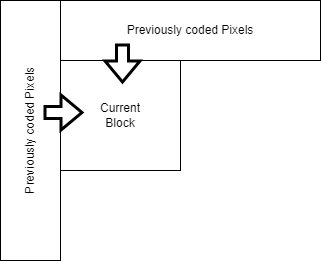
\includegraphics[width = 2.5in]{./Figures/comp1.png}
	\rule{35em}{0.5pt}
	\caption{Intra-Prediction}
	\label{fig:intraprediction}
\end{figure}

\subsection{Inter-Prediction}
Inter prediction is the process of predicting a block of luma and chroma samples from a picture that has been previously coded and transmitted i.e reference picture. It uses temporal sampling technique. For this, a prediction region is selected, then a prediction block is generated. After that the prediction block is subtracted from original block of samples to form a residual. The overview of the process is shown in figure \ref{fig:interprediction}.

\begin{figure}[htbp]
	\centering
	
\includegraphics[width = 3in]{./Figures/interprediction.png}
	\rule{35em}{0.5pt}
	\caption{Inter-Prediction}
	\label{fig:interprediction}
\end{figure}

\subsubsection{Motion Vector Prediction}
In video coding, motion vectors for neighboring partitions are typically closely related, and so each motion vector can be predicted using previously coded vectors from nearby partitions. A predicted vector is created based on these previous motion vectors, and the difference between the current vector and the predicted vector is encoded and transmitted. The way in which predicted vector is predicted depends on the size of the motion compensation partition and whether there are nearby vectors available for reference. For further details related to its algorithm and hardware development, refer to chapter \ref{Chapter4}.

\begin{figure}[htbp]
	\centering
	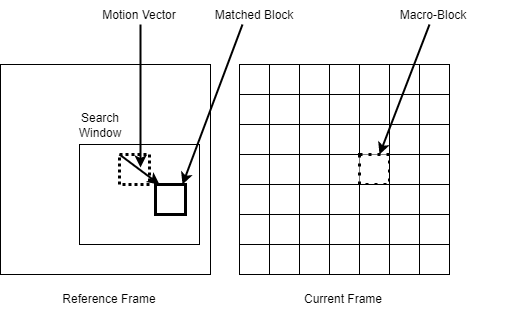
\includegraphics[width = 3in]{./Figures/motionvector.png}
	\rule{35em}{0.5pt}
	\caption{Motion Vector Prediction}
	\label{fig:motionvector}
\end{figure}

\subsection{Transform}
Once the residual data, which essentially comprises a block of residual coefficients, is obtained, it is subjected to the core transform process. This transform is an integer-based 4x4 or 8x8 transform that provides a scaled approximation to the Discrete Cosine Transform (DCT) \cite{richardson2010h264}. In certain cases, a portion of the output from this integer transform is subject to further transformation through a DC Transform, referred to as the Hadamard transform \cite{richardson2010h264}. The same residual data can be reconstructed using the DC inverse transform, which is carried out prior to rescaling. Finally, the rescaled coefficients are inverse transformed using a 4x4 or 8x8 inverse integer transform. To gain more insight of this process, refer to chapter \ref{Chapter3}.

\subsection{Quantization}
The transformed coefficients are subjected to quantization using a non-uniform quantizer. In this process, each coefficient is divided by an integer value, which reduces the precision of the coefficient values as determined by the Quantization Parameter (QP). The use of a non-uniform quantizer results in a smaller number of bits being used to represent each coefficient value, which in turn reduces the amount of data required to represent the video. The quantized transform coefficients of a block are typically scanned in a zig-zag pattern, which is a common approach for video coding standards. For more details, refer to chapter \ref{Chapter3}.


\subsection{Entropy Encoding}
In H.264 stream or file encoding, the symbols are coded in a series. The quantized transform coefficients are efficiently transmitted using the Context-Adaptive Variable Length Coding (CAVLC) method. The statistical distribution of the quantized transform coefficients typically shows larger values for low-frequency components that decrease gradually towards the high-frequency part. As a result, the number of nonzero quantized coefficients (N) and their size and position are coded separately. This enables the receiver to reconstruct the original signal more accurately. The coefficients are scanned in a zig-zag pattern, and then quantized to reduce their precision using the quantization parameter (QP). The efficient transmission of quantized transform coefficients in H.264 helps in reducing the size of the compressed video file while maintaining the quality of the video. The final Network Abstraction Layer can be seen in figure \ref{fig:syntax}. Further details of this implementation are mentioned in chapter \ref{Chapter3}.


% include h.264 syntax briefly
\section{H264 syntax}
H.264 consists of 2 layers: the \textbf{Network Abstraction Layer (NAL)} and the \textbf{Video Coding Layer (VCL)} \cite{richardson2010h264}. The NAL consists of a series of NAL Units, with \textbf{Sequence Parameter Sets (SPS)} and \textbf{Picture Parameter Sets (PPS)} being the most common units that signal certain control parameters to the decoder. In the VCL, coded video data is communicated in the form of slices.An \textbf{access unit}, which can be a coded frame or field, is made up of one or more slices. Each slice consists of a Slice Header and Slice Data, with the latter being a series of coded \textbf{macro blocks (MB)} and skip macro block indicators signaling that certain macro block positions contain no data.

\begin{itemize}
	\item \textbf{MB type:} I/intra coded, P/inter coded from one reference frame
	\item \textbf{Prediction information:} prediction mode for I macro block, choice reference frame and motion vectors for P macro block
	\item \textbf{Coded Block Pattern CBP:} indicates which luma and chroma blocks contain non zero residual co-efficient
	\item \textbf{Quantization Parameter QP:} for macro blocks with CBP not 0
	\item \textbf{Residual Data:} for blocks containing non-zero residual coefficients
\end{itemize}

The basic H264 syntax can be seen in figure \ref{fig:syntax}
\begin{figure}[htbp]
	\centering
	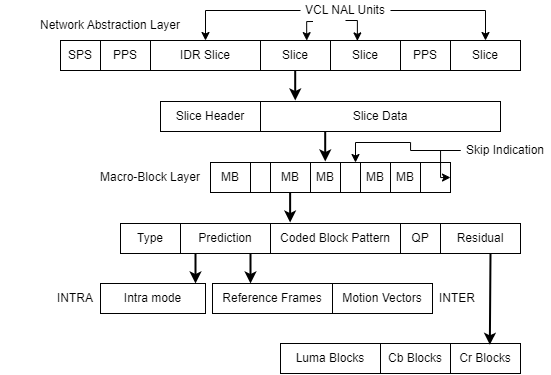
\includegraphics[width = 4in]{./Figures/syntax.png}
	\rule{35em}{0.5pt}
	\caption{Overall syntax for h264 encoder}
	\label{fig:syntax}
\end{figure}

In our project, we also successfully implemented the Baseline profile on FPGA board. The synthesis and the results obtained can be accessed in detail in chapter \ref{Chapter5}. The rest if the thesis is organized as follows:

Chapter \ref{Chapter2} gives an overview about the purpose of this project and mentions the problem statment of our project. Chapter \ref{Chapter3} explains Intra 4x4 luma and 8x8 Chroma Prediction. It also gives an overview of Inter prediction and its Block matching technique. Further the Transform coding, Quantization and Entropy Encoding and explained in detail. Chapter \ref{Chapter4} describes the Hardware Architecture for Inter Prediction in detail which is the main aim of our project. It explains the algorithm for carrying out the prediction of pixels. After that it explains the 256 PE VBS FS ME hardware architecture and its implementation in detail. Chapter \ref{Chapter5} follows with the simulation, results and the performance of the Baseline Profile and also the independent model of Inter Prediction. It also exhibits the implementation of Baseline Profile model of H.264 video encode on FPGA board and associated results. At last, the conclusion and future work are mentioned in Chapter \ref{Chapter6}.  % Introduction 

% Chapter 1

\chapter{Motivations and Problem Statement} % Write in your own chapter title
\label{Chapter2}
\lhead{Chapter 2. \emph{Motivations and Problem Statement}} % Write in your own chapter title to set the page header

\section{Motivations}

With the rapid increase in the development of products and services offering full-motion digital video, digital video coding is currently gaining importance and has a considerable monetary impact on computer, imaging and telecommunications technology.There have been a lot of efforts to achieve an efficient video encoding format, which offers a better remote viewing quality at a lower bit-rate and uses less bandwidth than the previous standards (i.e., MPEG-2, H.263, or MPEG-4 Part 2). H.264 or MPEG- Part 10 has all these new, better compression features that makes it more emphatic.The primary features that set H.264 apart from competing standards include network friendliness and good video quality at both high and low bit rates \cite{amer2005high}.

\section{Why H264 is more efficient?}

It is proposed that H264 can deliver two times better performance than the previous MPEG-2 coding standard, both in terms of compression efficiency and picture eminence. Moreover, previous H.63 and MPEG-4 implement block-based motion estimation to reduce temporal redundancy between frames. But in H.264, block matching efficiency is improved by some innovative features such as variable block size motion estimation (VBS$\_$ME) and motion vector prediction \cite{li2003serial}. The computational complexity of this model is increased by the factor of four due to these features.

\section{Project Continuation}

This is a \textbf{long-term project}, in collaboration with \textbf{10x Engineers} and team from \textbf{NUST}. A team from 10x worked on the ISP part of it whereas our group worked on the encoder part of the camera. This work is unique in Pakistan as very few engineers here work on SoC designs. This makes our project valuable as it can lead to new opportunities for local research and it can make a significant impact on the video compression industry and contribute to the development of new technologies in Pakistan and beyond.

\section{Need for further Improvements}

In terms of encoding efficiency and computational complexity, there is still a need for further improvements in the Baseline profile of H.264 especially if we are planning to use this standard for real time applications. Our contribution is a significant step towards enhancing the over-all performance of the CODEC i.e. by optimizing the inter-prediction algorithm to reduce the bit-rate and improve the visual quality of the video. 


 % What to Write 

% Chapter 1

\chapter{Prediction, Transformation, Quantization and Encoding} % Write in your own chapter title
\label{Chapter3}
\lhead{Chapter3. \emph{Prediction, Transformation, Quantization and Encoding}} % Write in your own chapter title to set the page header

\section{Prediction}
Prediction is defined as duplication of the information contained in a macro-block using previously coded data. This duplicated information is subtracted from the macro-block to form a residual. There are 2 types of prediction.

\begin{itemize}
	\item Intra-Prediction
	\item Inter-Prediction
\end{itemize}

% ref of intra+prediction paper
\subsection{Intra-Prediction}
Intra-prediction utilizes the space dependency to compress the video. The frames which are intra coded using intra-prediction are called I-frames. Following are the possible prediction modes:
\begin{itemize}
	\item \textbf{4x4 luma:} having 9 directional modes and is suitable for macro blocks that has lot of details
	\item \textbf{8x8 luma:} having 9 directional modes and is for high profiles only.
	\item \textbf{16x16 luma:} having 4 directional modes that is suitable for macro block with smoother area
	\item \textbf{8x8 chroma:} 4 possible prediction modes and used for chrominance components
\end{itemize}
In our model, 4x4 luma prediction and 8x8 chroma prediction is being implemented.

\subsubsection{4x4 Luma Prediction}
For this type of prediction, each macro block that is of \textbf{16x16} (256 pixels each of which is 8 bit wide) is divided into \textbf{4x4} block (16 pixels) \cite{anilkumar2021intra}. Figure \ref{fig:4x4xluma} shows the reference samples for 4x4 luma prediction. 4 pixels \textbf{A,B,C,D} (adjacent to current block) of block \textbf{a}  on top of current block, pixels \textbf{E,F,G,H} of block \textbf{b} on top right corner, \textbf{I,J,K,L} of block \textbf{c} at adjacent left of current block and 1 pixel \textbf{M} of \textbf{d} block on top left corner are used for prediction of 16 pixels in the current block.

\begin{figure}[htbp]
	\centering
	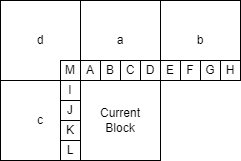
\includegraphics[width = 2.5in]{./Figures/4x4luma.png}
	\rule{35em}{0.5pt}
	\caption{Reference samples for 4x4 Luma}
	\label{fig:4x4xluma}
\end{figure}

There are total 9 prediction modes that are supported in this prediction. Major modes that are implemented in our model are as follows:

\begin{itemize}
	\item \textbf{Mode 0 (Vertical):} The predicted block is constructed by using upper samples A,B,C,D of block ‘a’ as shown in figure \ref{fig:3modes}. They are extrapolated vertically. It is suitable to predict vertical edges in the block.
	\item \textbf{Mode 1 (Horizontal):} In this mode, left samples I,J,K,L of block c are used. They are extrapolated horizontally and is suitable for horizontal edges. It can be seen in figure \ref{fig:3modes}.
	\item \textbf{Mode 2 (DC):} It utilizes average of all adjacent samples (A to D and I to L) to form the prediction of current block. It is suitable for smooth areas. Its process is shown in figure \ref{fig:3modes}.

\end{itemize}
	 
For the details of remaining modes refer to \cite{richardson2010h264}. Figure \ref{fig:3modes} display the above 3 prediction modes. To create a predict sample, every color stands for a particular formula. The encoder determines each prediction direction's cost by finishing processing for all of the prediction directions, then outputs the one with the lowest cost.

\begin{figure}[htbp]
	\centering
	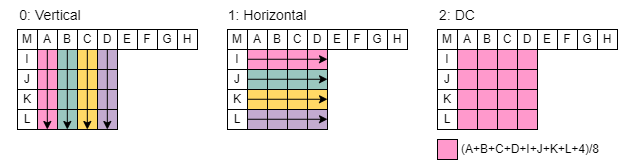
\includegraphics[width = 4in]{./Figures/3modes.png}
	\rule{35em}{0.5pt}
	\caption{Major Modes for 4x4 Luma Prediction}
	\label{fig:3modes}
\end{figure}

\subsubsection{8x8 Chroma Prediction}
This type of prediction applies on chrominance components. It is similar to 16x16 luma prediction which can be referred in \cite{richardson2010h264} except the block size is 8x8 and there is different order of mode number which are:

\begin{itemize}
	\item Mode 0: DC
	\item Mode 1: Horizontal
	\item Mode 2: Vertical
	\item Mode 3: Plane
\end{itemize}

The working of first 3 modes in similar to mode 2,1,0 of 4x4 luma prediction respectively. For details of Plane mode refer to \cite{richardson2010h264}. The Implemented mode in our model is DC. These modes are shown in the figure \ref{fig:8x8modes}.

\begin{figure}[htbp]
	\centering
	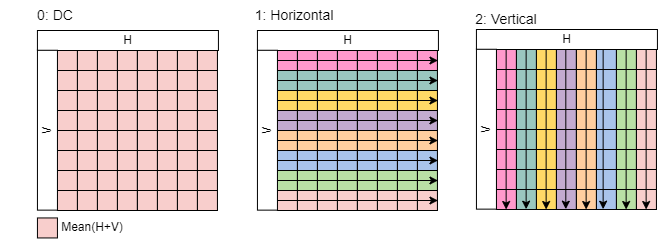
\includegraphics[width = 4in]{./Figures/8x8modes.png}
	\rule{35em}{0.5pt}
	\caption{Major Modes for 8x8 Chroma Prediction}
	\label{fig:8x8modes}
\end{figure}

%[Explain the hardware architecture of Intra prediction if possible]

\subsection{Inter-Prediction}
The process of predicting a block of luma and chroma samples from a reference picture that has been previously been coded and transmitted i.e. exploits temporal redundancy between successive frames. For this a prediction region is selected, a prediction block is generated and then it is subtracted from original block of samples to form a residual. This is then coded and transmitted. Reference pictures are stored in Decoded Picture Buffer. The offset between position of current block and search region in the reference picture is called motion vector. This prediction is also known as \textbf{Motion Estimation} \cite{kalaycioglu2011low}. It has the capability of extracting true motion information thus enhancing the quality of displayed images in video enhancement systems. The preferred technique for motion estimation is the \textbf{Block Matching (BM)} Technique. 


\subsubsection{Block Matching Technique}
This method divides the current frame into non-overlapping NxN macro-blocks and seeks out the block from the reference frame that most closely resembles the current block within a specified search range. The Sum of Absolute Difference (SAD), which is appropriate for hardware implementations, is the recommended block matching criterion.

In figure \ref{fig:mv}, \textbf{(x,y)} represents the location of the current frame. The search window in the reference frame is in \textbf{[-r,r]} region in both x and y directions. Both current and reference block lies within the range of search window. The SAD value is calculated by accumulating absolute differences of corresponding pixels in both current and reference blocks. A motion vector is the relative motion of current block in reference frame, they are specified in relative coordinates. Thus if \textbf{(x+a,y+b)} is the location of best matching block in reference frame, then \textbf{(a,b)} represents the motion vector. Motion Estimation is performed on luma component and resulting motion vectors are also used for chroma components.

\begin{figure}[htbp]
	\centering
	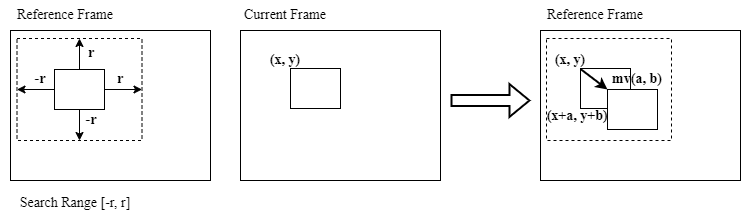
\includegraphics[width = 4in]{./Figures/mv.png}
	\rule{35em}{0.5pt}
	\caption{Motion Estimation using Block Matching}
	\label{fig:mv}
\end{figure}

There are several algorithms for Block Matching. Among them mostly used is \textbf{Full Search (FS)} algorithm. The SAD values for each search position within a specific search range are calculated by this approach to determine the reference block that most closely resembles the present block. It has the best performance related to other algorithms as it searches all the search locations in a given search range. But its computational complexity is high and its hardware consume a lot of power. For further improvement, instead of \textbf{fixed block size (FBS) FS ME} algorithm, \textbf{variable block size (VBS) FS ME} algorithm is incorporated. For details of FBS ME algorithm, refer to [that ppr]. VBS FS ME algorithm will be further explained in detail in chapter \ref{Chapter4}.


\section{Transform Coding}

\subsection{DC Transform}
The DC transform is a type of discrete cosine transform (DCT) that only operates on the DC component (i.e., the average pixel value) of a 2x2 input block, and it is used to reduce the amount of spatial redundancy in the video data.\\
This DC transform is a rather simple operation, it calculates the average of all the pixels in the input block, and then subtracts that average value from each pixel. The resulting values are then encoded and transmitted. For a 2x2 input block X, the sum of all the pixels is calculated as Given a 2x2 input block X, compute the sum of all the pixels in the block as: 

\begin{equation}
	SUM(X) = X(0,0) + X(0,1) + X(1,0) + X(1,1)
\end{equation}

The average value of the input block is computed as:

\begin{equation}
 AVG(X) = SUM(X) / 4
\end{equation}

then the average value is subtracted from each pixel in the input block to obtain the transformed block Y, where:
\begin{equation}
 	Y(i,j) = X(i,j) - AVG(X) 
\end{equation} 	
In our code this dc transform is implemented in a pipe-lined manner, i.e. by using 4 stages. In each stage the input block is first divided into two sub-blocks, the transform is applied to each sub-block then these transformed sub-blocks are recombined at the end to form the output block. This pipe-lining is done to ensure the reduced latency and higher throughput of transform. 

\subsection{Core Transform}
Core transform or Forward Discrete Cosine Transform (\textbf{FDCT}) is a linear transformation that transforms the given input data from spatial domain to frequency domain. This transform is \textbf{computationally less complex} and has \textbf{high energy compaction} as compared to \textbf{DFT}, \textbf{DST}, \textbf{WHT} and \textbf{DWT}. Therefore, it is highly preferred in video compression.
FDCT uses A i.e. a transform matrix and its transpose to convert the input matrix or a martix of samples X into a result matrix Y i.e. an NxN block of coefficients, as shown in the equation below:
\begin{equation}
	Y = AXA^{T}
\end{equation}
Here, A in an NxN transform matrix, the equation for $A_{ij}$ is given by:
\[
A_{ij} = C_i \cos\left(\frac{(2j + 1)i\pi}{2N}\right)
\]

where
\[
C_i = \begin{cases} 
	\frac{1}{\sqrt{N}} & \text{if } i = 0 \\
	\frac{\sqrt{2}}{\sqrt{N}} & \text{if } i > 0 \\
\end{cases}
\]

It can be simplified as a matrix, The matrix $A$ is given by:
\[
A = \begin{bmatrix}
	a & a & a & a \\
	b & c & -c & -b \\
	a & -a & -a & a \\
	c & -b & b & -c \\
\end{bmatrix}
\]

where
\[
a = \frac{1}{2}, \quad
b = \frac{1}{2}\cos\left(\frac{\pi}{8}\right), \quad
c = \frac{1}{2}\cos\left(\frac{3\pi}{8}\right)
\]

In our code, we have used 36-bit input, XXIN, which is a 4x9-bit matrix in little-endian order for our implementation of core transform. The transform generates a 14-bit output, YNOUT, in reverse zigzag order.\\
The output is only considered valid when the VALID signal is high. This VALID signal is controlled by the ENABLE signal. A READY signal that is used to indicate when the module is ready to accept input.\\
The output of core tranform is a set of coefficients in frequency domain, these coefficients, concentrate most of the signal energy in a few low frequency components. This property gives us efficient compression as the low magnitude coefficients are further discarded through quantization.

\section{Quantization}
The process of mapping the input values from a large set(typically a continuous set) into smaller often finite sized set is called Quantization. This helps in representing the data signal with fewer bits than the original one as the range of possible values in the quantized set in smaller.\\
We have used a \textbf{Scalar Quantizer} in our implementation, here each element on the matrix is quantized independently without considering the correlation between elements. For better understanding it can be considered as a process of rounding a fractional number to the nearest integer.\\
This process is irreversible and lossy since it is not possible to determine the exact value of the original fractional number from the rounded integer.\\
The formula used for quantization in our implementation is:
\[
X_q = \text{round}\left(\frac{X}{{2 \cdot QP}} \cdot \text{scale}\right)
\]
Here, \textbf{X} is the input value to be quantized. \textbf{QP} is the Quantization Parameter. The division by (2*QP) scales the input value based on the QP. \textbf{Scale} is the scaling factor and \textbf{round} function is used to round the scaled value to nearest integer, this scaled and rounded value is then multiplied by the scaled factor.

<<<<<<< Updated upstream
=======
\section{Encoding}
Variable Length Encoding is an encoding technique typically used in H.264 main profile, such encoder maps the input data into a series of code words, called variable length codes (VLCs). Each symbol corresponds to a codeword, which can vary in length but always has to have a fixed amount of bits. Short VLCs are used to represent frequently occurring symbols, while lengthy VLCs are used to represent less often occurring symbols. This results in data compression when there are enough encoded symbols in a given amount of data.

\subsection{Context Adaptive Variable Length Coding,CAVLC}
Context-Adaptive Variable Length Coding also known as CAVLC is a method coding transformed and quantized coefficients,it is an important component in video compression, particularly in the H.264 video coding standard. This encoding technique uses context adaptation to select various sets of variable-length codes based on the statistics of recently-coded coefficients.\\
High compression efficiency is attained by CAVLC by utilising the statistical characteristics of video data. It improves compression over fixed-length coding methods by adjusting the coding scheme based on the local context of the coefficients.\\
CAVLC effectively represents the quantized coefficients using variable length codes, lowering the bitrate of the compressed video stream. As a result, the video data is represented in more concise ways.\\
Compared to other entropy coding methods like CABAC (Context-Adaptive Binary Arithmetic Coding), CAVLC encoding and decoding processes are computationally simpler. As a result, real-time video encoding applications are better suited for it.\\
After transformation and quantization, blocks usually contain a lot of zeros, CAVLC uses run-level coding to represent this string of zeros compactly. A block of coefficients is converted into a series of variable length codes (VLCs) using zigzag scan (or field scan). The highest non-zero coefficients are often the sequence of +1 or -1 (called high frequency coefficients) and these are signaled by CAVLC as 'Trailing 1s' (T1s) in a compact way.\\
The number of non-zero coefficients in neighbouring blocks is correlated and this number is encoded with the help of a look up table. CAVLC encoding proceeds as follows:
\begin{itemize}
	\item First the lookup table encodes both number of non-zero coefficients and the number of Trailing 1s (T1s).
	\item Each T1 is signaled by lookup table, and the sign in encoded by a single bit i.e. 0 for '+' and 1 for '-', this is done in a reverse order starting from highest frequency T1.
	\item The sign and magnitude remaining non-zero coefficients is encoded in reverse order (from highest frequency back towards DC coefficients).
	\item Sum of all zeros before highest non-zero coefficient in the reverse ordered array is coded with a VLC.
	\item The number of zeros preceding each non-zero coefficient (run before) is encoded in reverse
	order.
\end{itemize}


>>>>>>> Stashed changes
 % Experimental Setup

% Chapter 1

\chapter{Hardware Architecture for Inter-Prediction} % Write in your own chapter title
\label{Chapter4}
\lhead{Chapter 4. \emph{Thesis Structure}} % Write in your own chapter title to set the page header

There are many new technologies such as intra prediction, in loop deblocking filter, context based arithmetic coding introduced in the latest H.264/AVC standard. Among all of these amazing technologies, \textbf{Variable Block Size Motion Estimation (VBSME)} is one of the powerful techniques. In comparison with the previous Fixed Block Size Motion Estimation (FBSME), VBSME divides one MB into smaller blocks to fit the different motion directions. In this way, the coding performance is proved.

\subsection{Full Search ME Algorithm}
The Full Search Algorithm works in the following way:
\begin{itemize}
	\item At first, both the search window and current block positions are fixed at the certain point i.e top left corner of frame. The current block starts the loading of the pixels from the top left corner. Absolute difference of each pixel of current block with the corresponding pixel of the search window is calculated.
	\begin{equation} \label{equ:1}
		Diff(m,n,k,l\ = |S(m+k, n+l) - C(k,l)|
	\end{equation}
	\item After that the Sum of all Absolute Differences (SAD) for that particular position of current block is calculated.
	\begin{equation} \label{equ:2}
		SAD(m,n) = \sum_{k=0}^{W-1}\sum_{l=0}^{H-1}Diff(m,n,k,l) 
	\end{equation}
	Then the current block is shifted by 1 row or column of pixels and again SAD is calculated. In this way, several SADs are calculated in a single search window.
	\item Each SAD when calculated is compared with the previous SAD value and the smaller SAD value is taken. In this way at end, minimum SAD value and the corresponding motion vectors values are depicted for one search window. 
	\begin{equation} \label{equ:3}
		SAD_{min} = min(SAD(m,n))
	\end{equation}
\end{itemize}

In the above equation (\ref{equ:1}), (\ref{equ:2}) and (\ref{equ:3}) The domain of m and n is $m \in [0, M-1] $ and $m \in [0, N-1]$ respectively.M and N are width and height of search window respectively. H and W are height and width of current block respectively. C(k,l) represents the pixel value of the current block and S(m+k, n+l) is the pixel value from the search window of the reference frame.\cite{li2003serial} \\

\subsection{256 PE VBS FS ME Hardware Architecture}
We designed a parallel \textbf{256 PE VBS FSME Hardware Architecture}. \cite{kalaycioglu2011low} This hardware is implemented in System Verilog. First of all, the pixels in the current MB are stored in a Block Ram \textbf{(c$\_$BRAM)}. The pixels of the search window are also stored in a block RAM \textbf{(s$\_$BRAM)}. The architecture is shown in the figure \ref{fig:256pevbsme}

\begin{figure}[htbp]
	\centering
	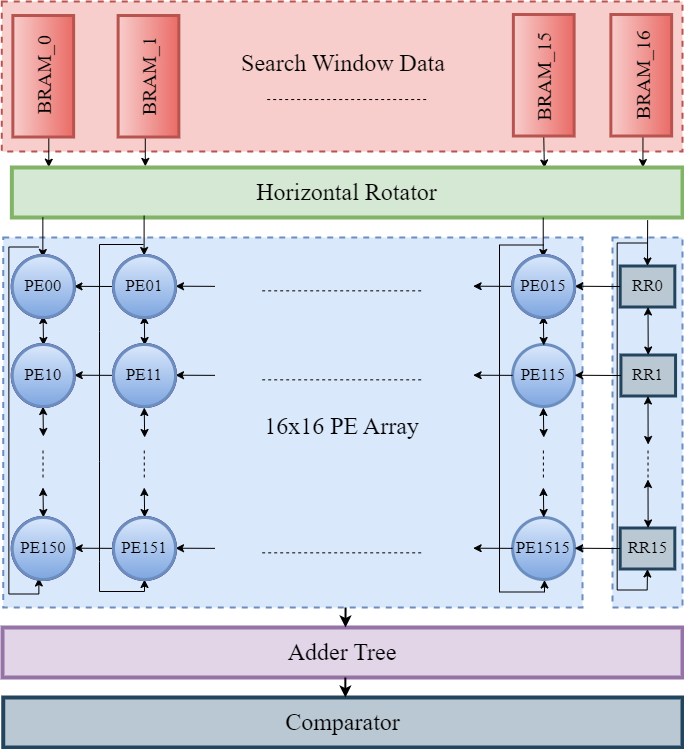
\includegraphics[width = 4in]{./Figures/256pevbsme.png}
	\rule{35em}{0.5pt}
	\caption{265 PE VBS ME Hardware Architecture}
	\label{fig:256pevbsme}
\end{figure}

In this design, a \textbf{2-D systolic PE array} is used. The use of this type of array introduced parallel computing and pipelinability in the structure. There are \textbf{16x16 = 256 PEs} ( 16 rows and 16 columns) interconnected with each other in a form of matrix. All of them are  made capable of shifting data down, up and left. It means that a 16x16 current block can move around the 48x48 search window in down, up and right direction. For a \textbf{16x16 MB}, a Motion Vector MV is found in one cycle in a search range of \textbf{[-16, 15]} pixels. Pixels are defined as 8 bit positive integers.

As soon as the control signals for loading current and search pixels are enabled, both current block and search window pixels starts loading into PEs. In 1 clk cycle, 16 pixels are loaded for both of them. (1st PE is filled in each of 16 columns). Thus, the whole PE matrix is filled in 16 cycles. As depicted in figure \ref{fig:pematrix}, \textbf{pixel$\_$cpr$\_$in} and \textbf{pixel$\_$spr$\_$in} are input array of 16 8-bit pixels from current block and search window of reference block respectively. The \textbf{pe$\_$}matrix module concatenates the output signals of each column of processing elements to form the final output signal \textbf{ad} which is an array of 8*(16**2) bits. 

\begin{figure}[htbp]
	\centering
	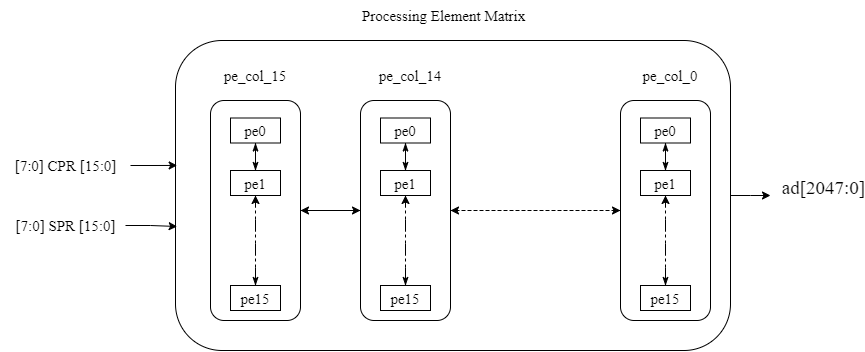
\includegraphics[width = 4.5in]{./Figures/pematrix.png}
	\rule{35em}{0.5pt}
	\caption{16 x 16 PE Matrix}
	\label{fig:pematrix}
\end{figure}

Each PE calculates the absolute difference between current MB pixel and the search window pixel. In this way 16x16 = 256 absolute differences are obtained in one location and they all are calculated simultaneously with the loading of data in PEs as the design is combinational. 

After absolute differences are all calculated, The SAD for that search location is determined by adding the absolute differences calculated by the above PEs as shown in figure. All these absolute differences are added up together using Adder Trees. The working of a simple adder tree is shown in figure \ref{fig:addertree}. It can seen clearly in the figure that there is 2 cycle latency for an adder tree. 

\begin{figure}[htbp]
	\centering
	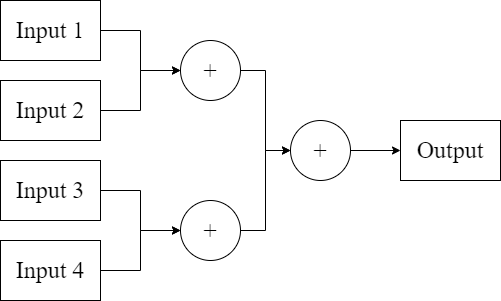
\includegraphics[width = 2in]{./Figures/addertree.png}
	\rule{35em}{0.5pt}
	\caption{Working of an Adder Tree}
	\label{fig:addertree}
\end{figure}

For SAD calculation of a 16x16 current block, we consider \textbf{PI-PPSAD} structure.  

 % Experiment 1

% Chapter 1

\chapter{Results and Performance} % Write in your own chapter title
\label{Chapter5}
\lhead{Chapter 5. \emph{Results and Performance}} % Write in your own chapter title to set the page header


\section{Performance Evaluation of H.264 Encoder}

\subsection{Effect of Different Values for QP}
In order to check the effect of quantization parameter on encoded video, the H.264 encoder is simulated using various values of QP. These results have been tabulated using a raw video of size \textbf{43.5 MB}.
\begin{table}[H]
	\centering
	\begin{tabular}{|c|c|c|c|c|} \hline
		\textbf{QP}  & \textbf{Encoded Video Size (MB)} & \multicolumn{3}{|c|}{\textbf{SNR (dB)}}  \\
		\cline{3-5}
		    &                    &  \textbf{Y} & \textbf{U} & \textbf{V}\\ \hline
		20  &    6.79            & 42.26   & 46.04  & 46.15  \\ \hline
		28  &    3.46            & 36.24   & 41.50  & 41.83  \\ \hline
		35  &    1.93            & 31.47   & 37.25  & 37.00  \\ \hline
	\end{tabular}
	\caption{Size and quality of encoded video for different QP values.}
	\label{tab:qp}
\end{table}
As discussed earlier in Chapter \ref{Chapter3}, the \textbf{Quantization Parameter} in quantization module determines to what extent the video should be compressed. A higher value of QP implies more compression, hence the size of encoded video is reduced but at the cost of poor video quality. The loss of information can be seen by reduced SNR values in the Table \ref{tab:qp}. On the contrary, a lower value of QP enhances the quality of video but at the expense of greater video size. Therefore, a moderate value for QP should be selected between 20-30 so that none of the metrics (size and quality) is compromised. 


\subsection{Resource Utilization}
The H.264 encoder is synthesized and implemented using Vivado for Xilinx Artix-7. The resource utilization for this module is shown below.
\begin{table}[H]
	\centering
	\begin{tabular}{|c|c|c|c|} \hline
		\textbf{Resource} & \textbf{Used} & \textbf{Available} & \textbf{Utilization\%}  \\ \hline
		Look Up Tables & 4214 & 63400 & 6.65 \\ \hline
		Registers 	  & 2578 & 126800 & 2.03 \\ \hline
		F7 Muxes      & 227 & 31700 & 0.72 \\ \hline
		F8 Muxes      & 72 & 15850 & 0.45 \\ \hline 
		Block RAM Tile & 2 & 135 & 1.48 \\ \hline
		DSPs & 2 & 240 & 0.83 \\ \hline
		Input/Output   & 90 & 210 & 42.86 \\ \hline 
	\end{tabular}
	\caption{Resource utilization of H.264 encoder for Artix-7.}
	\label{tab:resource_ec}
\end{table}
From the table \ref{tab:resource_ec} it is evident that all the resources comply with the Artix-7 specified limits. 
   
\section{Performance Evaluation of Inter-Prediction Module}
As stated in Chapter \ref{Chapter4}, the inter-prediction module developed for this project employs a 256 PE VBS ME hardware architecture. Thie module uses a datapath-controller design which is shown in the Figure \ref{fig:mehardware}. This schematic is generated using Vivado. 
\begin{figure}[H]
	\centering
	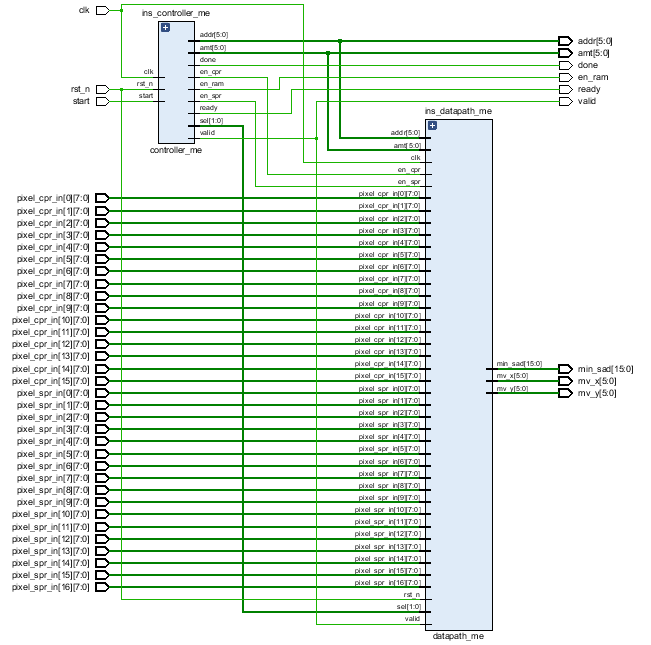
\includegraphics[width = 3in]{./Figures/mehardware.png}
	\rule{35em}{0.5pt}
	\caption{Schematic for inter-prediction module.}
	\label{fig:mehardware}
\end{figure}
\subsection{Resource Utilization}
The module for inter-prediction is analyzed and synthesized using Vivado for Xilinx Artix-7. The resource utilization for this module is shown below.
\begin{table}[H]
	\centering
	\begin{tabular}{|c|c|c|c|} \hline
		\textbf{Resource} & \textbf{Used} & \textbf{Available} & \textbf{Utilization\%}  \\ \hline
		Look Up Tables & 7376 & 63400 & 11.63 \\ \hline
		Registers & 7266 & 126800 & 5.73 \\ \hline
		Input/Output & 311 & 210 & 148.10 \\ \hline 
	\end{tabular}
	\caption{Resource utilization of inter-prediction module for Artix-7.}
	\label{tab:resource_me}
\end{table}

It can be seen from the results above that the utilization of look up tables and registers is within limits but the input/output has exceeded from the available resources. This issue is due to the fact that inter-prediction block has been synthesized separately. Once this module is integrated within the H.264 top module, the input/output ports will be reduced sufficiently.  

\subsection{Simulation Results}
In order to verify the working of inter-prediction module, it is simulated using a MB of size 16x16 from the current frame and a search range of size 48x48 from the reference frame.
The loading of MB takes 16 cycles and after that the pixels of search range are loaded in the RAMs. It takes 16 cycles to calculate the first valid SAD value as the RAMs are getting filled for the first time. Once the first valid SAD value is calculated the next values are calculated with no latency. This is due to the fact that RAMs are filled and only the shifting of pixels need to be done which is done by BRAM 16 as seen in Figure \ref{fig:256pevbsme}. Therefore, this architecture reduces the latency for SAD calculation. This can also be verified by the following simulation waveform.
\begin{figure}[H]
	\centering
	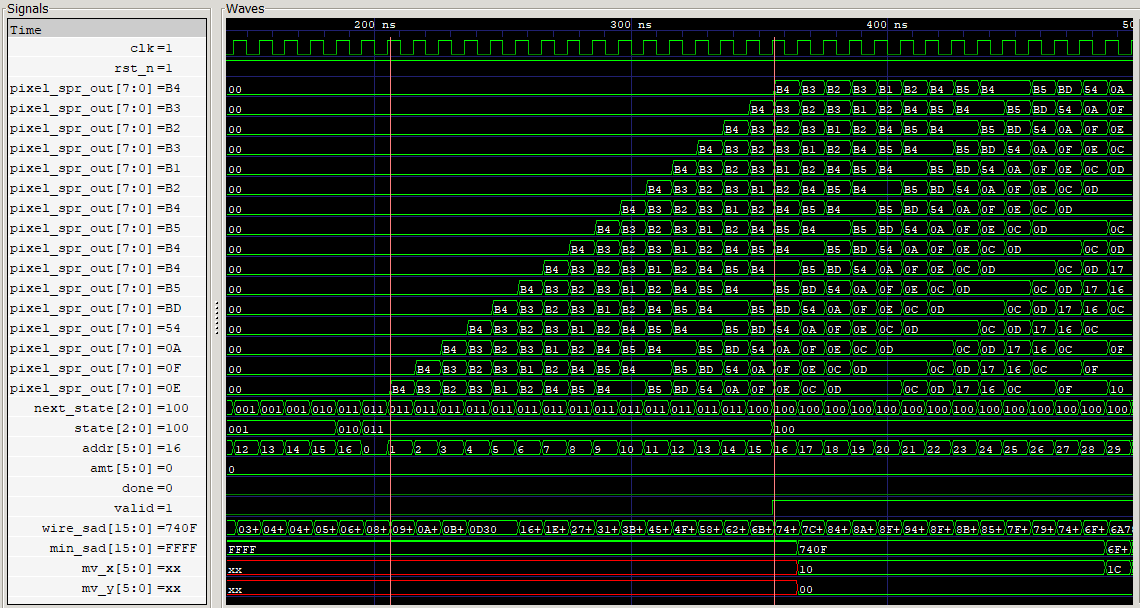
\includegraphics[width = 4in]{./Figures/wave3.png}
	\rule{35em}{0.5pt}
	\caption{Simulation waveform of inter-prediction module for one search range (a).}
	\label{fig:wave3}
\end{figure}
Once the MB has traversed the search range, it asserts a signal done and the final values for motion vectors in x and y direction, corresponding to the minimum SAD value are obtained. 
\begin{figure}[H]
	\centering
	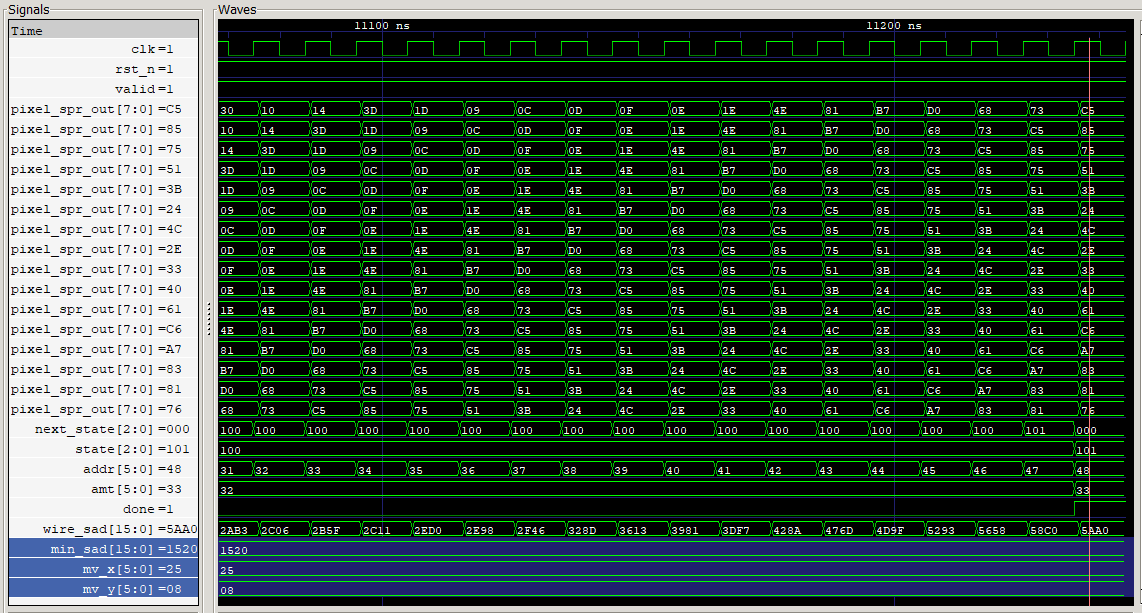
\includegraphics[width = 4in]{./Figures/wave2.png}
	\rule{35em}{0.5pt}
	\caption{Simulation waveform of inter-prediction module for one search range (b).}
	\label{fig:wave2}
\end{figure}

 % Experiment 2

% Chapter 1

\chapter{Thesis Structure} % Write in your own chapter title
\label{Chapter1}
\lhead{Chapter 1. \emph{Thesis Structure}} % Write in your own chapter title to set the page header

The flow of information provided in a thesis depends on its structure. The parameters defining the structure of a thesis are discussed in \cite{getthesis} and are quoted below:  

\begin{quote}
``The structure of a thesis is governed by logic and is invariant with respect to subject. The substance varies with subject, and its quality is determined by the technical knowledge and mastery of essentials exhibited by the student. Style has two components: language and layout. The former deals with the usage of English as a medium of sound technical communication; the latter with the physical presentation of the thesis on paper. All three components structure, substance and style influence one another."
\end{quote}

There is no definite structure for a thesis. The author is the best judge. One possible structure of a thesis can be:

\begin{itemize}
	\item \textit{Chapter 1}: Introduction
	\item \textit{Chapter 2}: Motivations, Related Literature and Problem Statement
	\item \textit{Chapter 3}: Proposed Approach
	\item \textit{Chapter 4}: Implementation and/or Experimentation 
	\item \textit{Chapter 5}: Conclusions and Future Directions 
\end{itemize}

The purpose of the introduction is to provide an outline of your project in a contextual framework systematically. The introduction should be kept short and to the point. 

Depending on the substance, you can break Chapter 2 suggested above into  separate chapters. For instance, \textit{motivation and related literature} can be one chapter and \textit{problem statement} can be a separate chapter . This is flexible and is decided while writing the thesis. 

The rationale behind the structure selected above is to meet the objective of telling a story as clearly and convincingly as possible. We have adapted the following table from \cite{barrass2002scientists} to show the flow in the logic:

\begin{table}[h]
\centering
\begin{tabular}{l|l} \hline
Introduction/Aim  & What did you do and why? \\
Materials and Methods & How did you do it? \\
Observations/Results & What did you find? \\
Discussion & What do your results mean to you and why? \\
Conclusions & What new knowledge is extracted from experiment? \\ \hline
\end{tabular}
%\caption{Flow in the logic}
\label{tab:logic_flow}
\end{table}


There are a number of guiding documents e.g. \cite{murray2006write}, \cite{evans2003write}, as well as some documents available online, which can be helpful in writing the thesis. Two such documents outlining some general guidelines are \cite{howtothesis}, \cite{getthesis}.

Finally here is a list of words that you should try avoid while writing the thesis: ``very much", ``interesting", ``good", ``fun", ``exciting", ``very", ``too much".




 % Results and Discussion

%% Chapter 1

\chapter{Thesis Structure} % Write in your own chapter title
\label{Chapter7}
\lhead{Chapter 7. \emph{Thesis Structure}} % Write in your own chapter title to set the page header

The flow of information provided in a thesis depends on its structure. The parameters defining the structure of a thesis are discussed in \cite{getthesis} and are quoted below:  

\begin{quote}
``The structure of a thesis is governed by logic and is invariant with respect to subject. The substance varies with subject, and its quality is determined by the technical knowledge and mastery of essentials exhibited by the student. Style has two components: language and layout. The former deals with the usage of English as a medium of sound technical communication; the latter with the physical presentation of the thesis on paper. All three components structure, substance and style influence one another."
\end{quote}

There is no definite structure for a thesis. The author is the best judge. One possible structure of a thesis can be:

\begin{itemize}
	\item \textit{Chapter 1}: Introduction
	\item \textit{Chapter 2}: Motivations, Related Literature and Problem Statement
	\item \textit{Chapter 3}: Proposed Approach
	\item \textit{Chapter 4}: Implementation and/or Experimentation 
	\item \textit{Chapter 5}: Conclusions and Future Directions 
\end{itemize}

The purpose of the introduction is to provide an outline of your project in a contextual framework systematically. The introduction should be kept short and to the point. 

Depending on the substance, you can break Chapter 2 suggested above into  separate chapters. For instance, \textit{motivation and related literature} can be one chapter and \textit{problem statement} can be a separate chapter . This is flexible and is decided while writing the thesis. 

The rationale behind the structure selected above is to meet the objective of telling a story as clearly and convincingly as possible. We have adapted the following table from \cite{barrass2002scientists} to show the flow in the logic:

\begin{table}[h]
\centering
\begin{tabular}{l|l} \hline
Introduction/Aim  & What did you do and why? \\
Materials and Methods & How did you do it? \\
Observations/Results & What did you find? \\
Discussion & What do your results mean to you and why? \\
Conclusions & What new knowledge is extracted from experiment? \\ \hline
\end{tabular}
%\caption{Flow in the logic}
\label{tab:logic_flow}
\end{table}


There are a number of guiding documents e.g. \cite{murray2006write}, \cite{evans2003write}, as well as some documents available online, which can be helpful in writing the thesis. Two such documents outlining some general guidelines are \cite{howtothesis}, \cite{getthesis}.

Finally here is a list of words that you should try avoid while writing the thesis: ``very much", ``interesting", ``good", ``fun", ``exciting", ``very", ``too much".




 % Conclusion

%% ----------------------------------------------------------------
% Now begin the Appendices, including them as separate files

\addtocontents{toc}{\vspace{2em}} % Add a gap in the Contents, for aesthetics

\appendix % Cue to tell LaTeX that the following 'chapters' are Appendices

% Appendix A

\chapter{Computation of DCT}
\label{AppendixA}
\lhead{Appendix A. \emph{Computation of DCT}}

The Discrete Cosine Transform (DCT) is a widely used transformation technique in signal processing and data compression. It converts a sequence of input values into a set of frequency coefficients, which represent the signal's energy in different frequency bands. 
Following is the step-by-step computation of the DCT for a 3x3 matrix.

Step 1: Define the input matrix
\[
\mathbf{A} = \begin{bmatrix}
	a_{1,1} & a_{1,2} & a_{1,3} \\
	a_{2,1} & a_{2,2} & a_{2,3} \\
	a_{3,1} & a_{3,2} & a_{3,3} \\
\end{bmatrix}
\]

Step 2: Subtract the mean from the matrix
\[
\bar{\mathbf{A}} = \begin{bmatrix}
	a_{1,1} - \mu & a_{1,2} - \mu & a_{1,3} - \mu \\
	a_{2,1} - \mu & a_{2,2} - \mu & a_{2,3} - \mu \\
	a_{3,1} - \mu & a_{3,2} - \mu & a_{3,3} - \mu \\
\end{bmatrix}
\]
where \(\mu\) is the mean value of the elements in matrix \(\mathbf{A}\).

Step 3: Compute the DCT coefficients
\[
\mathbf{B} = \begin{bmatrix}
	b_{1,1} & b_{1,2} & b_{1,3} \\
	b_{2,1} & b_{2,2} & b_{2,3} \\
	b_{3,1} & b_{3,2} & b_{3,3} \\
\end{bmatrix}
\]
where
\[
b_{i,j} = \sum_{x=1}^{3} \sum_{y=1}^{3} \bar{a}_{x,y} \cdot \cos\left(\frac{(2x-1)(i-1)\pi}{6}\right) \cdot \cos\left(\frac{(2y-1)(j-1)\pi}{6}\right)
\]
for \(i,j = 1,2,3\).

Step 4: Normalize the DCT coefficients
\[
\mathbf{C} = \begin{bmatrix}
	c_{1,1} & c_{1,2} & c_{1,3} \\
	c_{2,1} & c_{2,2} & c_{2,3} \\
	c_{3,1} & c_{3,2} & c_{3,3} \\
\end{bmatrix}
\]
where
\[
c_{i,j} = \frac{1}{\sqrt{2N}} \cdot b_{i,j}
\]
for \(i,j = 1,2,3\) and \(N\) is the size of the matrix (in this case, \(N = 3\)).

	% Appendix Title

%\input{./Chapters/AppendixB} % Appendix Title

%\input{./Chapters/AppendixC} % Appendix Title

\addtocontents{toc}{\vspace{2em}}  % Add a gap in the Contents, for aesthetics
\backmatter

%% ----------------------------------------------------------------
\label{References}
\lhead{\emph{References}}  % Change the left side page header to "References"

\bibliographystyle{plainnat}  % Use "unsrtnat" BibTeX style for formatting the references

\bibliography{references}  % The references information are stored in the file named "references.bib"

\end{document}  % The End
%% ----------------------------------------------------------------
